\section{Task 5}

\subsection{Overview of Clenshaw's algorithm}

Clenshaw's algorithm evaluates a polynomial in Chebyshev form with \( O(n) \) complexity. Compared with standard polynomial evaluation, its recursive treatment significantly accelerates computation.

The experiment compared Clenshaw's algorithm with classical Chebyshev-polynomial evaluation. The plot shows mean runtimes for both methods. Settings were as in Task 1.

\subsection{Results and conclusions}

\begin{center}
\textbf{Mean time for Clenshaw's method:} \( 0.000578 \pm 0.000324 \)
\textbf{Mean time for the standard method:} \( 0.000692 \pm 0.000393 \)
\textbf{Speedup:} \( 1.20 \times \pm 0.03 \times \)
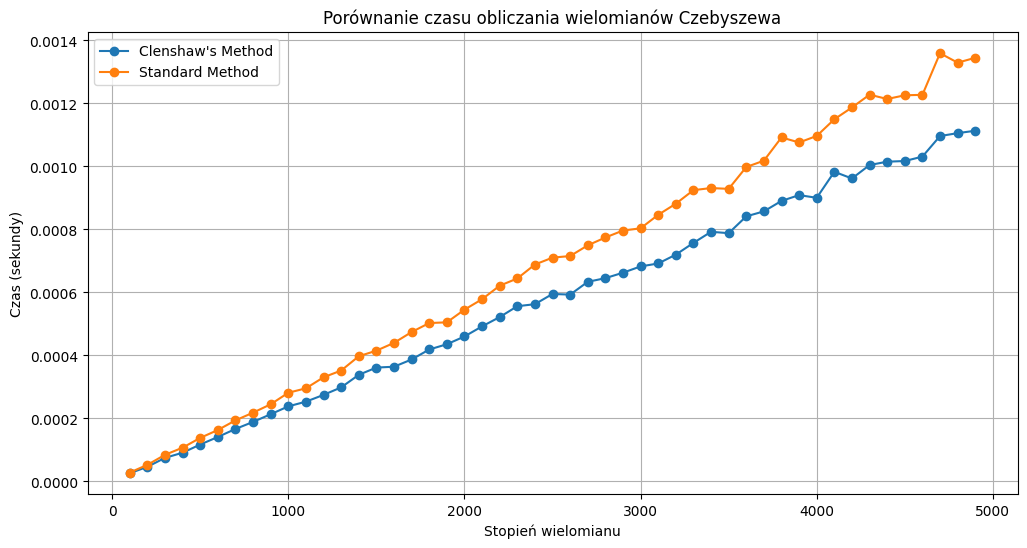
\includegraphics[width=\textwidth]{figures/task-4/chebyshev_5000.png}
\end{center}

\textbf{Conclusions:}
\begin{itemize}
    \item \textbf{Speed of Clenshaw's method:} Clenshaw's algorithm clearly outperforms standard Chebyshev-polynomial evaluation, running an average of 1.20x faster.
    \item \textbf{Comparison with Horner:} Clenshaw's method approaches the optimal runtime known from Horner's algorithm, which is a special case for Chebyshev polynomials.
    \item \textbf{Runtime stability:} Unlike Horner's algorithm, Clenshaw's method does not exhibit runtime fluctuations, indicating greater numerical stability.
\end{itemize}
